\documentclass{article}
\usepackage[utf8]{inputenc}

\title{Lecture 4: Significance Tests }
\author{wbg231 }
\date{November 2022}
\usepackage{tikz,graphicx,amsmath,amsfonts,amscd,amssymb,bm,cite,epsfig,epsf,url}
\begin{document}

\maketitle

\section{introduction}
\subsection{outline for the null hypothesis framework}
\begin{itemize}
%\item 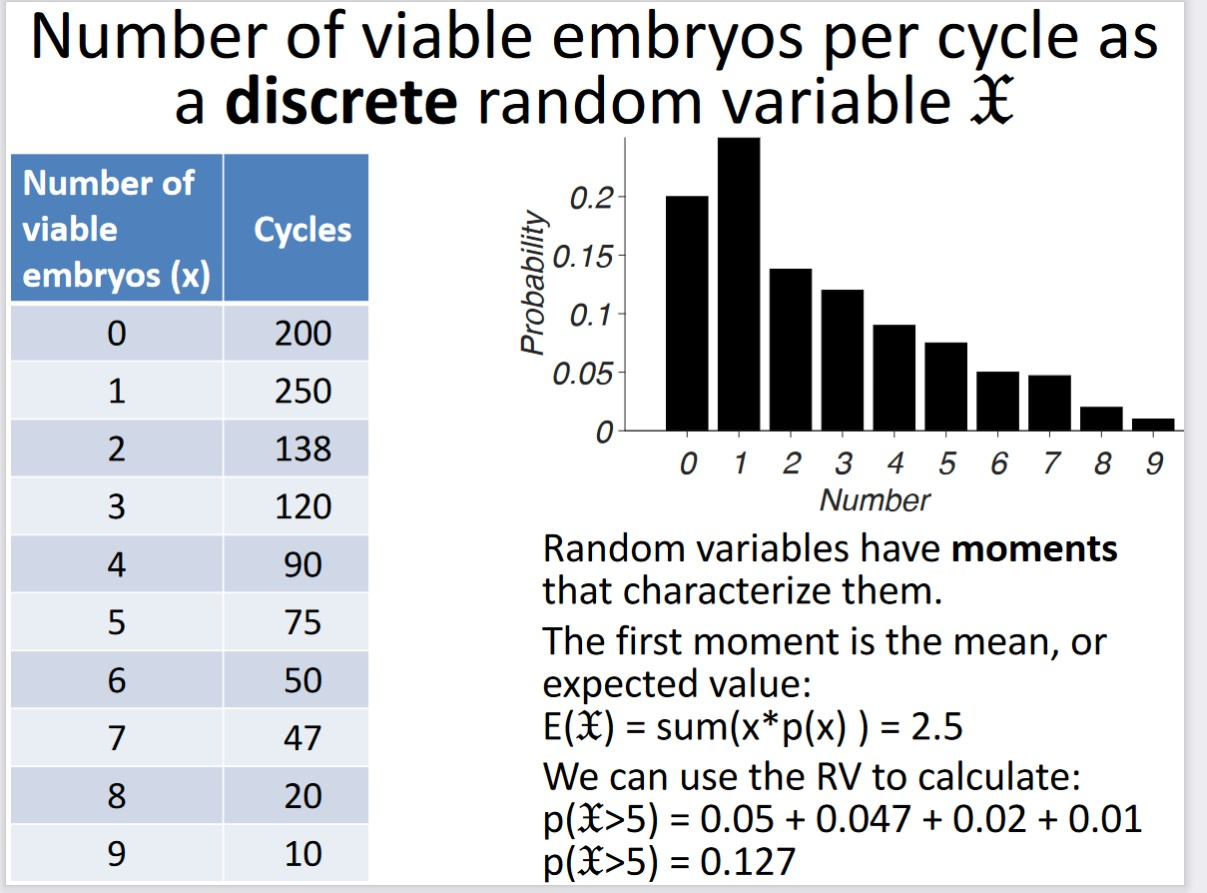
\includegraphics[width=7.5cm]{Final_Review/Lecture_2/lecture_1example.jpg}
\item start by proposing a hpyoshis with a treatment. 
\item we then assume that the treatment has no effect (ie the null hypnotises is true
\item then we measure the outcome of the treatment group and those of the control group
\item then we compare the outcomes in the two groups recognizing that any difference could be caused by chance
\item if the difference in outcomes are two large to be caused by Chance alone we reject our assumption that the null is true
\item if the difference in outcomes could be found by chance, then we can not conclude anything 
\item we are making a choice, descions can be wrong 
\item this framework is the predominate approach in industry and science 
\item science at this point is predominately p values, and there are many in industry as well. 
\item p valeus are in well over half of the papers. that are published.
\item today we are going over difrent use cases and when to use which test 
\subsection{Sign Test}
\item this is the oldest test 
\item this is mostly for historical intrest. 
\item it was intorduced by john arbuthnot
\item the question it was dessined to awnser was are male and female birth equally likely 
\item he assuemd the null that they are euallty likely
\item he looked at london birth records and the number of male and females 
\item he found that the probaility of that quantity of males assuming that the null is true rare so more males are both 
\item we see male births more because, male sperm is lighter? 
\item he interpreted this result as god providing since, more males die in war, so you can be right about the statistics but have bad conclusions 
\item this works well with discrete outcomes 
\subsection{Z test intorduction}
\item not everyhting is countable 
\item we want to know if a drug increases iq 
\itme our null is this drug does not improve iq 
\item in the general population the iq is known to be normally distributed and the populaiton mean is 100 adn the popoulationn standard devaiton is 15. this is how iq was defined. 
\item these are the condtions for when we are able to do a z test. 
\item we know waht the expecation should be 
\item we give the drug to 25 people and test there outcomes 
\begin{enumerate}
    \item $\me=100, \sigma=15$ n=25
    \item our question is did this new sample come from our null population (ie the normal iq destitution) 
    \item we calcualte a sample mean $\Bar{X}=109$
    \item so now we want to know how likley is it to get this sample mean. 
    \item \frac{109-100}{\frac{15}{5}}=3
    \item we know that z scores 
    \item p=.03
    \item that is less than alpah so we reject the null
\end{enumerate}
\item the z vlaue is calucalted as $z=\frac{\Bar{x}-\mu}{\text{SEM}}=\frac{\Bar{x}-\mu}{\frac{\sigma}{\sqrt{n}}}$
\item recall that SEM is teh standard error of the mean. in other words we are normalizing how far our sample mean is from the populaiton mean, by the standard error of the sample mean. this formla $x_{sd}=\frac{x-\mu_x}{\sigma_x}$ is how we standardize varibales to be distributed betwene 0 and 1.
\item since  we know that sample means are normally distributed by the CLT, we know that $z$ will be normally distributed between [0,1]
\item then we convert the z value to a p value and compare that to our $\alpha$
\subsection{ Where does the p-value come from }
\item we need to transofmr the z value to a probaility
\item we know that z is normal zero 1 distributed so we can find the p value as the likylyhood of finding a vlaue as or more extreme than this vlaue 
\item a one tailed test means we are only interested in if $\alpha$ raises or lowers the quantity in one direction that has an alpha of 1.65
\item if we want a two tailed test then we just care about the difference so cut of of plus or minus 1.96
\item two tailled tests are more conservative. 
\subsection{Z score as a test stat}
\item z score can be calucated as $z=\frac{x-\mu}{\sigma}$ is a standard way to normalize data. 
\item here we are using z sscores as a test statistic. 
\item so the question becomes how far is the observed sample mean from the population mean (if the null is true) in units of standard error of the mean. 
\item in normally distributed case things work out well.
\item the z score how ever is this $z=\frac{\Bar{x}-\mu}{\text{SEM}}=\frac{\Bar{x}-\mu}{\frac{\sigma}{\sqrt{n}}}$
\item teh standard normal distribute is well know so we can readily convert a z value to a probability 
\subsection{Z test full}
\item I am just going to run through the full logic of the Z test. 
\item so here we are int rested in if some sample comes from a normal distribution (ex does taking a drug raise iq) 
\item our null hypothesis is that the sample is from the normal distribution we know (that is the drug has no effect and people are on the normal iq distribution)
\item our alternative is that those who take the drug are unlikely to come from the known uniform null distribution ( ie that taking the drug makes you smarter
\item so we calculate our test statistic the z score as $z=\frac{\Bar{x}-\mu}{\text{SEM}}=\frac{\Bar{x}-\mu}{\frac{\sigma}{\sqrt{n}}}$
\item the numerator is the sample mean minus the null populaiton mena 
\item the denomiator is the stnadrd error of the sample mean. (more or less the standard devation of our sample means as a random varibale) 
\item so the z score distributes nomrally between 0 and 1, and represnets how many units of standard divation of the sample mena or observed data is form the population mean 
\item then we convert this to a p score, that is see if the area greater than or equal to this value under the pdf of the normal zero one standard distorbuiton is above our sigfngance level. this is our p-value
\item if it is above alpha we fail to reject teh null
\item if our p-value is bellow alpah we reject the null as the chance of the data being this different i sunlikely to oocour just do to sampleing error alone 
\subsection{confusion matrix }

\item  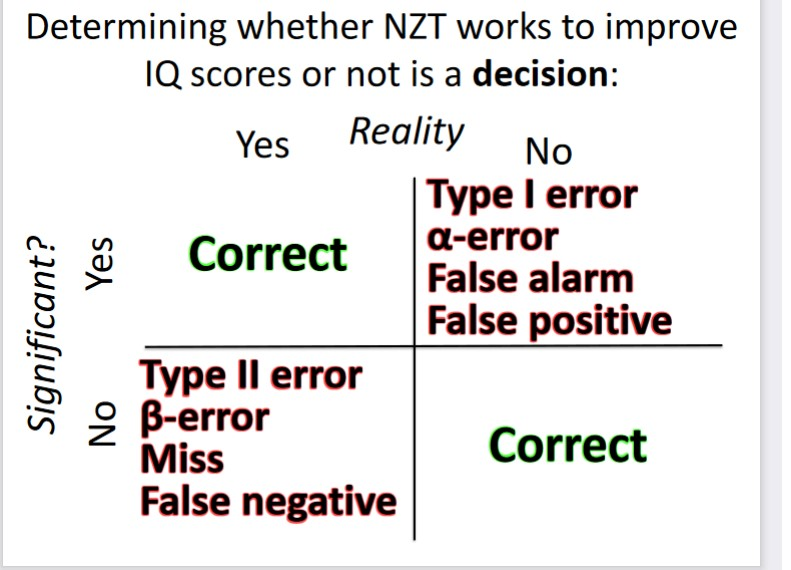
\includegraphics[width=7.5cm]{Final_Review/lecture_4/lecture 4 confusion_matrix.jpg}
\item we have made a descion case 1, sigfant in reality and the test 
\item case 2 clasify it as sifgngant but it is not we call that tpye 1 erorr, or $\alpha$ erorr. this is due to sampleing erorr. it can be controlled by the alpha level (on a per test bassis)
\item case 3 the drug does work in reality but, we could not detec tit that is called type 2 error. this is contorlled by statistical power
\item case 4 it does not work adn we conclude it does nto work, bad for the company good for society
\item data science is generally designed to avoid type 2 error. 
\item think of this in terms of a fire allarm. a tpye 2 error menas there is a fire and we do not notify poeple of this. 
\item descions can be wrong 
\item false postive: a person can be wronglyly executerd this happend in reality.
\item false negative: not recognizing that plains coming into peral harbror were going to attack, this happend in reality. 
\item it all depends on the context. 
\subsection{summary so far}
\item we want to know how likely our smaple is assuming chance alone 
\item to calculate this probaility we conver the sample mean to a test statsitic with a known null distribution (ie a distrobution given the null hpyothsis is ture) 
\item a test stat needs a known null distor
\item the p vlaue is the area under this null that is cut off by the test stat 
\item then we compare this value alpha 
\item in a z test. the z score is the test stat the normal (0,1) distobutioion is our null distobuiton 

\subsection{ when does z not work}
\item we usually do not know the population mean and standard deviation 
\item this also rellies on the central limit therome, so small samples do nto work 
\item enter the t test whcih avoids both of this 
\item the t test is the most commonly used test to analyze data form a/b designs 
\item but first must thinking about degrees of freedome 
\subsection{degrees of freedome}
\item this tends to be overlooked 
\item it is pretty straightforward once understood but it is 4 concepts that need to be understood.
\item where does hte name come from 
\begin{enumerate}
\item this does come up during job interviews sometimes 
\item item this comes form degrees of freedoms in pyhsics
\item a trian has 1 degree of freedom it can go back and forward 
\item a plain has 3 degres of freedome x,y,z
\item the name comes from rotaitonal axis ie directions in which you can movie
\end{enumerate}
\item what is the meaning in statitcs
\begin{enumerate}
    \item it is the number if independint pieces of indomration (numbers, measumrents, datapoints) in a dta set that a parameter calcualtion can be based on 
    \item the higher it is the more stable our estimate is 
    \item think about rate my prof, with prof A has higher rating with lower n, prof b has lwoer rating with higher n. \item it is more liekly that b is repreantivie
    \item degree of freedom is efective sample size
\end{enumerate}
\item how are they lost 
\begin{enumerate}
\item  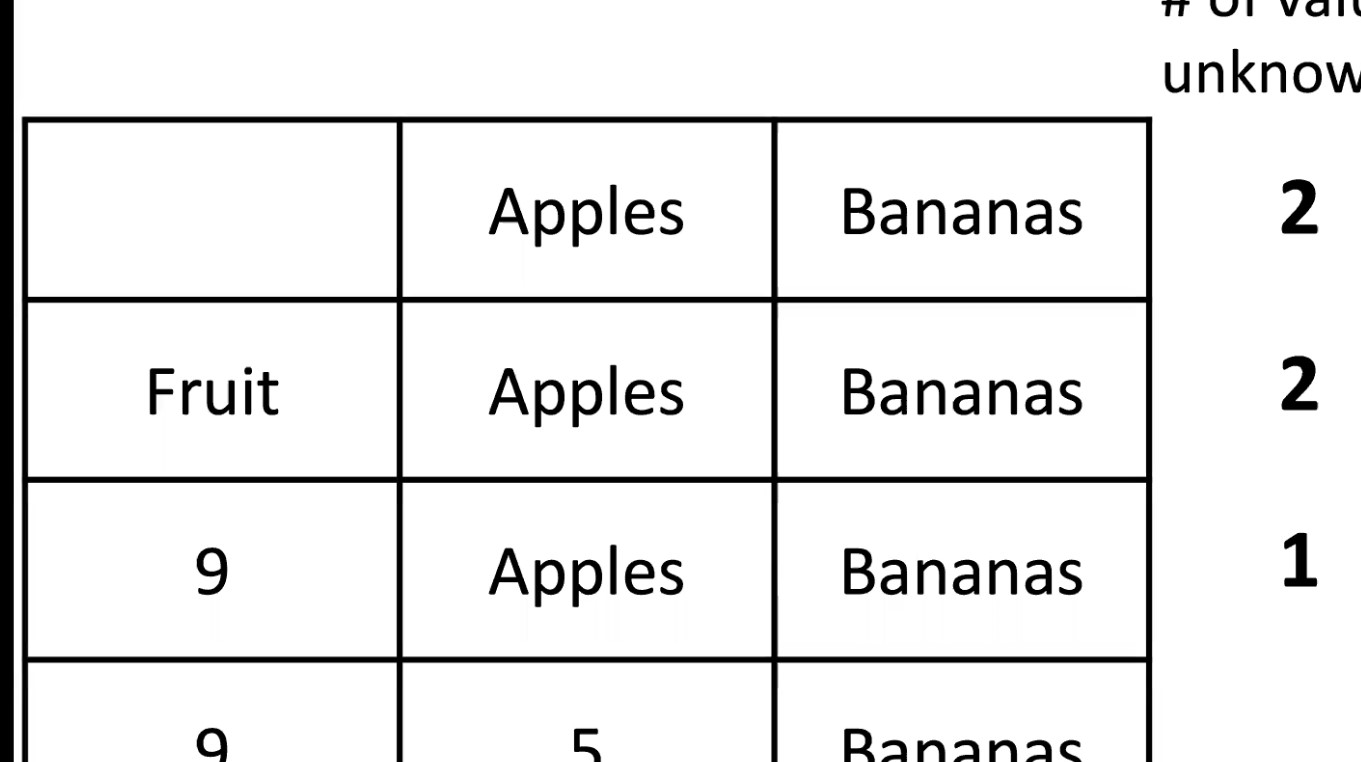
\includegraphics[width=7.5cm]{Final_Review/lecture_4/df_example.jpg}
\item only measuremnts create inpdendint informaiton, calcualtions corleate the infomraiton 
    \item think of data as random varibles
    \item have apples and banas thus have to random vairbles both are unknown 
    \item create a new rv called fruite that is apples +bananas. so there are still only 2 random vairbles that can freely varry.
    \item if we know that fruit =9 then we know that banana =9-apples so only either apples or banans can vary ie we only have 1 unknown quantity. 
    \item if both apples and fruit are set then there are 0 degrees of freedom 
\end{enumerate}
\item why does this matter
\begin{itemize}
    \item in practice we use the sample standard devation. not the populaiton standard devation 
    \item say we have a population of 5 numbers then we can calcaulte teh standard devation of the population as $\sigma=\sqrt{\frac{\sigma){i=1}^{n}(x_{i}-\mu)^2}{n}}$
    \item but are taking a sample we do not have the population mean we need t calculate the same $\Bar{X}=\frac{\Sigma_{i=1}^{n}x_i}{n}$ but notice that there is a summation in this. 
    \item so when we are calculating the sample standard deviation we need to adjust for the fact that we have summed already thus sample SD $ s=\sqrt{\frac{\sigma){i=1}^{n}(x_{i}-\Bar{x})^2}{n-1}}$
    \item so this is per parameter that we replace with the sample stat, so we lose 1 degree of freedom per sample mean we calculate. 
    \item df is not n-1
    \item degrees of freeom is n-k where n is the number of data points and k is the number iof paramters that are esiamted form teh samepl
    \item so in a case like A-NOVA this thing varries. 
\end{itemize}
\subsection{T test introduction}
\item \item  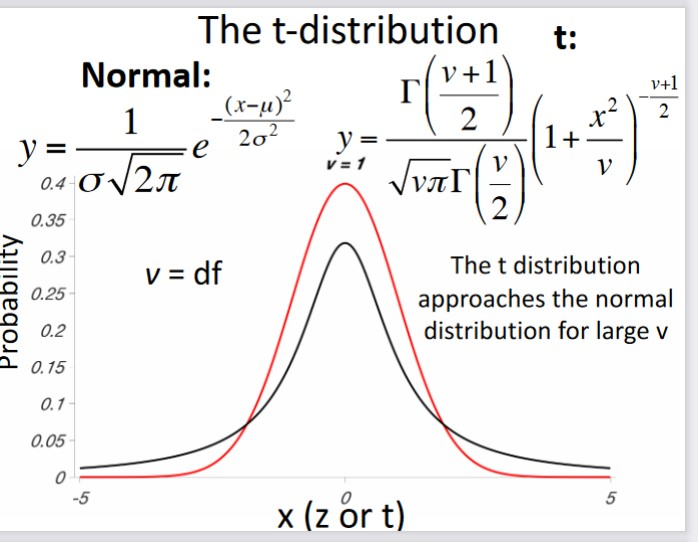
\includegraphics[width=7.5cm]{Final_Review/lecture_4/T_dsit.jpg}
\item $\Gamma$ (gamma) is basically factorial
\item the normal dist has 2 parameters mean and sd 
\item the gamma function has onyl 1 paramter $\nu$ representing degrees of freedom.  
\item as $\nu$ (ie degrees of freedom) aproahces inflinty the t distrobution aproaches the normal distrobution. it is pretty close after like 30 degrees of freedome 
\item at lower degrees of freedom, the distro is heavy tailled, meaning that extreme outcomes are more likely than in the normal distribution 
\item so t works for small sample sizes. 
\itme the z requires a large sample size
\item the t test also works with what you get from teh sample its self it does not need anyhtign from teh sample 
\subsection{student t test }
\item there was gosstet who published under a psydonm as student he leaked the secret to testin guiness beer 
\item the secret eis it works for smlal smapels with unkonw popualtion aprameters 
\item his use case was beer, how do you know that beer is good (dont know how it distributes ,cnat test it all )
\item $t=\frac{\Bar{X_1}-\Bar{x_2}}{SEM}$ this thing distributed as t/ 
\item so you dont need the population mean any more 
\item SEM in this case is pooled standard error 
\item you just need to look at the diference between the two sampels 
\item $x_1, x_2$ are samples that are treated difrently 
\subsection{logic of the test}
\item we dont know the popoualtion mean 
\item but we draw and comapre to samples and see if the treated and untreated sampels come from difrent populations 
\item this requires new assumptions 
\subsection{assumptions }
\item first it assuems that the mean can be intrepted normally
\item they assueme that the data is distibuted nroamlly
\item to meaningfulyl intrept a difnrece in teh samples by comparing the means the variability within each sample needs to be similar 
\item if the assumptions are violated, then the test does nto really work 
\item if you change the mean you usually change the variance so other tests are usually better
\subsection{there are several version of this test}
\item there are a few types 
\item firs the indedint groups t test
\begin{enumerate}
    \item also called between subject design 
    \item that is the true groups are disjoint you wieht get treamtemetn a or b which is sellected at random 
    \item  the degrees of freedom are $df=n-2$
    \item this is because we are calcuating $t=\frac{\Bar{X_1}-\Bar{x_2}}{SEM}$ this thing distributed as two sample means 
\end{enumerate}
\item then there is the t test for corelated groups (also called the paird sampels or dependint samples t- test) 
\begin{enumerate}
    \item this has a within subject design 
    \item here we test the same people twice once in condition one once in condition 2. 
    \item the samples are no longer independent they are litterly the same people. 
    \item so in this case we use the t test for corealated groups 
    \item we calcualte this t-score as $t=\frac{\bar(x_1-x_2)}{SEM_d}=\frac{\bar{D}}{SEM_d}$ where $\bar{D}$ is the mean of the difrence between eahc individual in treatment 1 and 2 
    \item we are only caluating one mean so the degrees of freedome ar e$df=n-1$
\end{enumerate}
\subsection{example}
\item work as a data sceintist want to test if a drug increases recation time. 
\item can only make 3 of the drug.
\item first try t test with indie groups 
\begin{itemize}
    \item group 1 3 poelpe wwith otut eh drug 
    \item group 2 poeple with teh drug 
    \item n=6 df=2
    \item $\sigma_{pool}=353$
    \item $SEM_{pool}=288$
    \item $T_{indpendint}=\frac{\bar{x_1}-\bar{x_2}}{sem_{pool}}=\frac{2000-1500}{288}$ then we convert to a p-vlaue 
    \item our p vlaue is p=.16 
    \item so in other wrods we find that the result is not sigfant 
    \item what kills us is there is a lot of variblly between indivudals that is being indepnedinted as variblei
    
\end{itemize}

\item paried t test
\begin{itemize}
    \item same data 
    \item n=3
    \item df=1
    \item $t=\frac{\bar{X}}{SEM_{d}}=\frac{500}{57.5}$
    \item this yields a p vlalue less than .05 so we conclude that the data works
\end{itemize}
\item if we have the opttion likely use the paired t test. 
\item even though we lost some degrees of freedom it is a stornger test.
\subsection{T test Summary}
\item here we want to test the difference between two groups. 
\item we need the means to be intrepreitbale 
\item we also need the variance within eaehc group to be similar 
\item we also need to asusme that the data is normally distributed 
\item the t distrovution only depends on the degrees of freedome. it is our null distorbution 
\item our test stat is t the t score. 
\item the indepdenint sampels t-test lets us calulate the difrence between two sampels that are disjoint.$t=\frac{\Bar{X_1}-\Bar{x_2}}{SEM}$ using this 
\item the dependint t test lets us caluate the difrence for a sample before and after a treatment like this $t=\frac{\bar(x_1-x_2)}{SEM_d}=\frac{\bar{D}}{SEM_d}$ where $\bar{D}$ is the mean of the difrence between eahc individual in treatment 1 and 2 
\subsection{Welsche T test }
\item this works better if varinace between groups is not homoginious 
\item it is a modfied version of the independint samples t test hat doe snot asusme homgenotiy of varinace 
\item it is bassically just working on the math if we do not assume the variance is equal 
\item the degrees of freedom need to be apromaited and they depdnint on size of each sample adn the stnadard deviation fo eahc sample
\item we might get fractional degrees of freedom 
\item the welche test gives lower degrees of freedom, then the t-test, so you need a larger n to get the same p-value, but it allows us to avoid assuming that we know the varince of the groups of the si simialr 
\item it is the best test to use though 
\subsection{anova}
\item this is for when we wnat to compare mroe than two gorups 
\item he skips it here but there is a lecture on it, that we should watch 
\item the logic is it extends the logic of the t test to mroe than two groups. 
\item it is mathamatically equivlent to regression. it is the GLM model effectivly  \item so far all our of sigfgance test rellie on the sample mean being meaninfull 
\subsection{when the mean does not make sense}
\item the obvious case is catagorical data. the mean of tow cartagories does not mean anyhting 
\item instead we can count how oftena  catagory shows up in our dataset what can we do with counts
\subsection{$\chi^2$ tests}
\item$\chi^2$ test should be avoided if possible it loses a lot of power
\item someitmes this is all we can do with catagorical data
\item so we just use the count of the number of each catagory that appears as opposed to means
\item so we dont lose any degrees of freedome 
\item it is the least powerfull test
\item it is a non-parametric test that just compares the distrobtion of catagoricla data 
\item it makes fewer assumption, but is a bit weeker. 
\item so we bassically look if the count of the catagorial changes between the two groups
\subsection{example}
\item is zodaic sign predictive of beign a ceral killer
\item sereal killers are more likely to be cerial killers.
\item so lets view zodiaks as catorigal data 
\item null hypothsis there difrrence in number of cereal killers based on birth sign 
\item have a dataset of 360 killers with there date of bith 
\item we can look at there empyrical distrobution. scorpyos are the most common sign in the sample (the marginal)
\item but what is the cahnce of seing such a high ressutl by chance? 
\item we can not do this with any test but the $\chi ^2$
\item so we compare the expected catagory coutns to the empyrical catagory counts we square the difrneces and sum tehm up that is teh test stat $\chi^2=\Sigma\frac{\text{(observed count - expected count})^2}{\text{expected count }}$
\item we know the $\chi^2$ distributes so we can use that test to caluate how likly it is under the null, ie what is the area under the null 
\item the test stat $\chi^2$ is a function of the numebr of catagories. \item in the zodiac case we haev 
\item the marginal is the expected count
\item so we go over all the classes. 
\item so there are 12 classes 
\item so the df is the number of classes minus the numebr of marginal 
\item the marignal is the expected count 
\item so in this case we have 12 classes 1 marignla and thus 11 degrees of freedom 
\item so teh issue was caused by sampleing variability
\item anyhting that involved ordinal data otehr test
\subsection{ordinal data}
\item the mean only works if the unit size is equal but ordinal data like starts does not have the same distance
\item teh distnace between 2 and 3 starts may not be the same as 3 and 4 starts for isntance 
\item so we need a test that works with ordinal data instead of a t-test
\item this is where the man-whiteney u enters 
\item there is also an issue with ergodicity. 
\item if we sample from a unfirom distrbutioon with  a large n we get a nroaml dsitrbution of smaple emans 
\item but waht if the population has some extreme values 
\item if we sample from a distrobution that has really large extreme values the means are not deffined (so cauchy distorbutions) mean we cant use tests based on teh sample mean 
\item the cauchy is non-ergotic
\subsection{Mann-Whiteney U test}
\item also called wilcoxon rank sum test.
\item works well for cases when there are extreme values, or ordinal data. 
\item basscially test if the two sampels come form distributiosn withteh same mendian 
\item the median is robust to outliers ,and distance between types does not matter
\item the test stat is the U, this has a know null distro
\item so we calcaulate an empyrical u, then see what perctange of null is cut off by our observed u 
\subsection{basic idea}
\item we have data from two sampels
\itme we arange both samples toghter in rank order
\item if both samples came form teh same underlying distribution there should Be ranodm mixing and the sum fo the rnaks should be simialr for both sampels
\item otherwise there should be a difrnec ein teh sum of these ranks 
\item but is is possible for two distrobutions to have the same median but be dsitributed difrent 
\subsection{Kolmogrov- smirnov test}
\item jsut ussualy called the ks test 
\item the idea is that we are not comparing medians or modes but instead the whole distorbution 
\item we are comapting the cumultiative distorbution empyrically
\item we try to see how well do the CDFs between samples fit 
\item we are integrating the area under the pdf from the left. 
\item so regardless of what the cdf is we know they go form 0 to 1, so we can find the point of largest sepration adn use that as our test statsitic D
\item 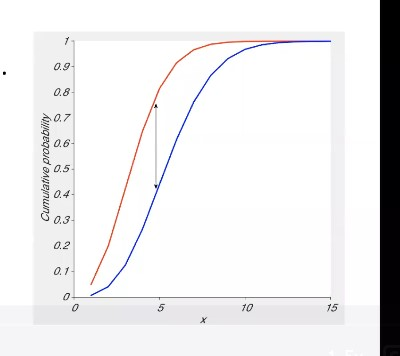
\includegraphics[width=7.5cm]{Final_Review/lecture_4/KS_1.jpg}
\item the ks test is versatile can use it with literly anyhting 
\item it usses a single point, so it is not very stong though. 
\subsection{Kruscal wallace test}
\item this is the anova but non parametric 
\subsection{null hyptoshis tesitng step by step}
\begin{enumerate}
    \item state the null hypothsis assume it is true 
    \item impement a reaserch design to test it
    \item pick a test to do (no matter what test you do you get a test stat) 
    \item then take the test stat and get a p value 
    \item is that p value SMALLER than alpha?
    \item if yes reject our assumptuon that the null hyptoshsis is ture 
    \item if no dont rejec the asusmption that the null hpyothsis is true
\end{enumerate}
\subsection{When to use which test}
\item this is kind of the job picking the best test to use when and why 
\item here is a descion tree
\item 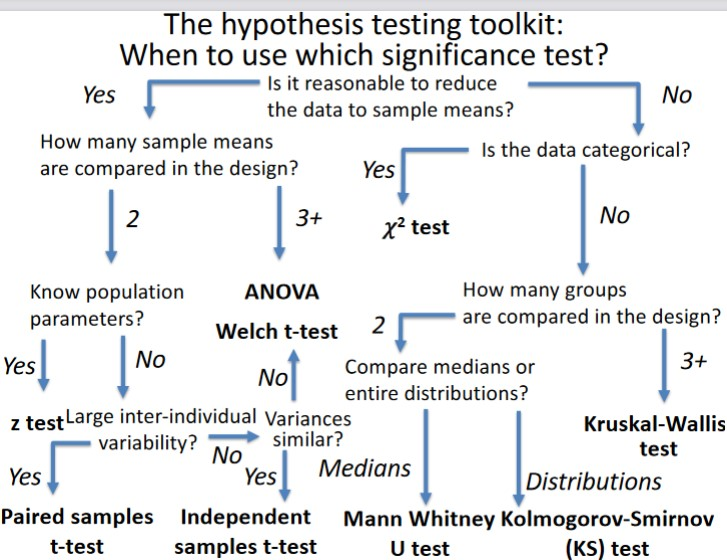
\includegraphics[width=7.5cm]{Final_Review/lecture_4/hypothis tesitng tool kit.jpg}
\item question 1. can the data be reduced to its sample means 
\item if yes go elft these are the parametric side of the test
\item how many sampel emans are we comapring if more than 2 use anova
\itme if the number of groups is 2 go left 
\itme if we know the popualtion aprmaeters use z tes t
\item if not we use the t tests
\item if there is large inter individual viarbleility use the paired sample t test 
\item if we dont think ther eis large inter indiuval vairbles. if the varinace is simalr use a indepndint samples t test
\item if the variance is not simialr use the welshe t test
\item now we want to go through non-parmaetirc this is if the mena does not make snese, that is oridnal catagorical and extreme valeus 
\item if the test is catagorila use chi squared
\item if we are comparing three or more sampels we use the ks test 
\item is we have exactly two and we are comparing medianas we use mann whiteny
\item if we have 2 and we are comparing distroburtions we use the ks test
\item that ends lecrue 4 matrerial pick up in the lecture 5 vedio 30 minutes in 
\end{itemize}

\end{document}
